\documentclass{article}

\usepackage{graphicx}
\usepackage{tikz}
\usepackage{tikzsymbols}
\usetikzlibrary{calc,patterns,shapes.geometric}
\pagestyle{empty}
\usepackage[margin=0pt]{geometry}
\geometry{papersize={14in,12in}}

\def\centerarc[#1](#2)(#3:#4:#5){\draw[#1] ($(#2)+({#5*cos(#3)},{#5*sin(#3)})$) arc (#3:#4:#5);}

\begin{document}
	\begin{figure}
		\centering
		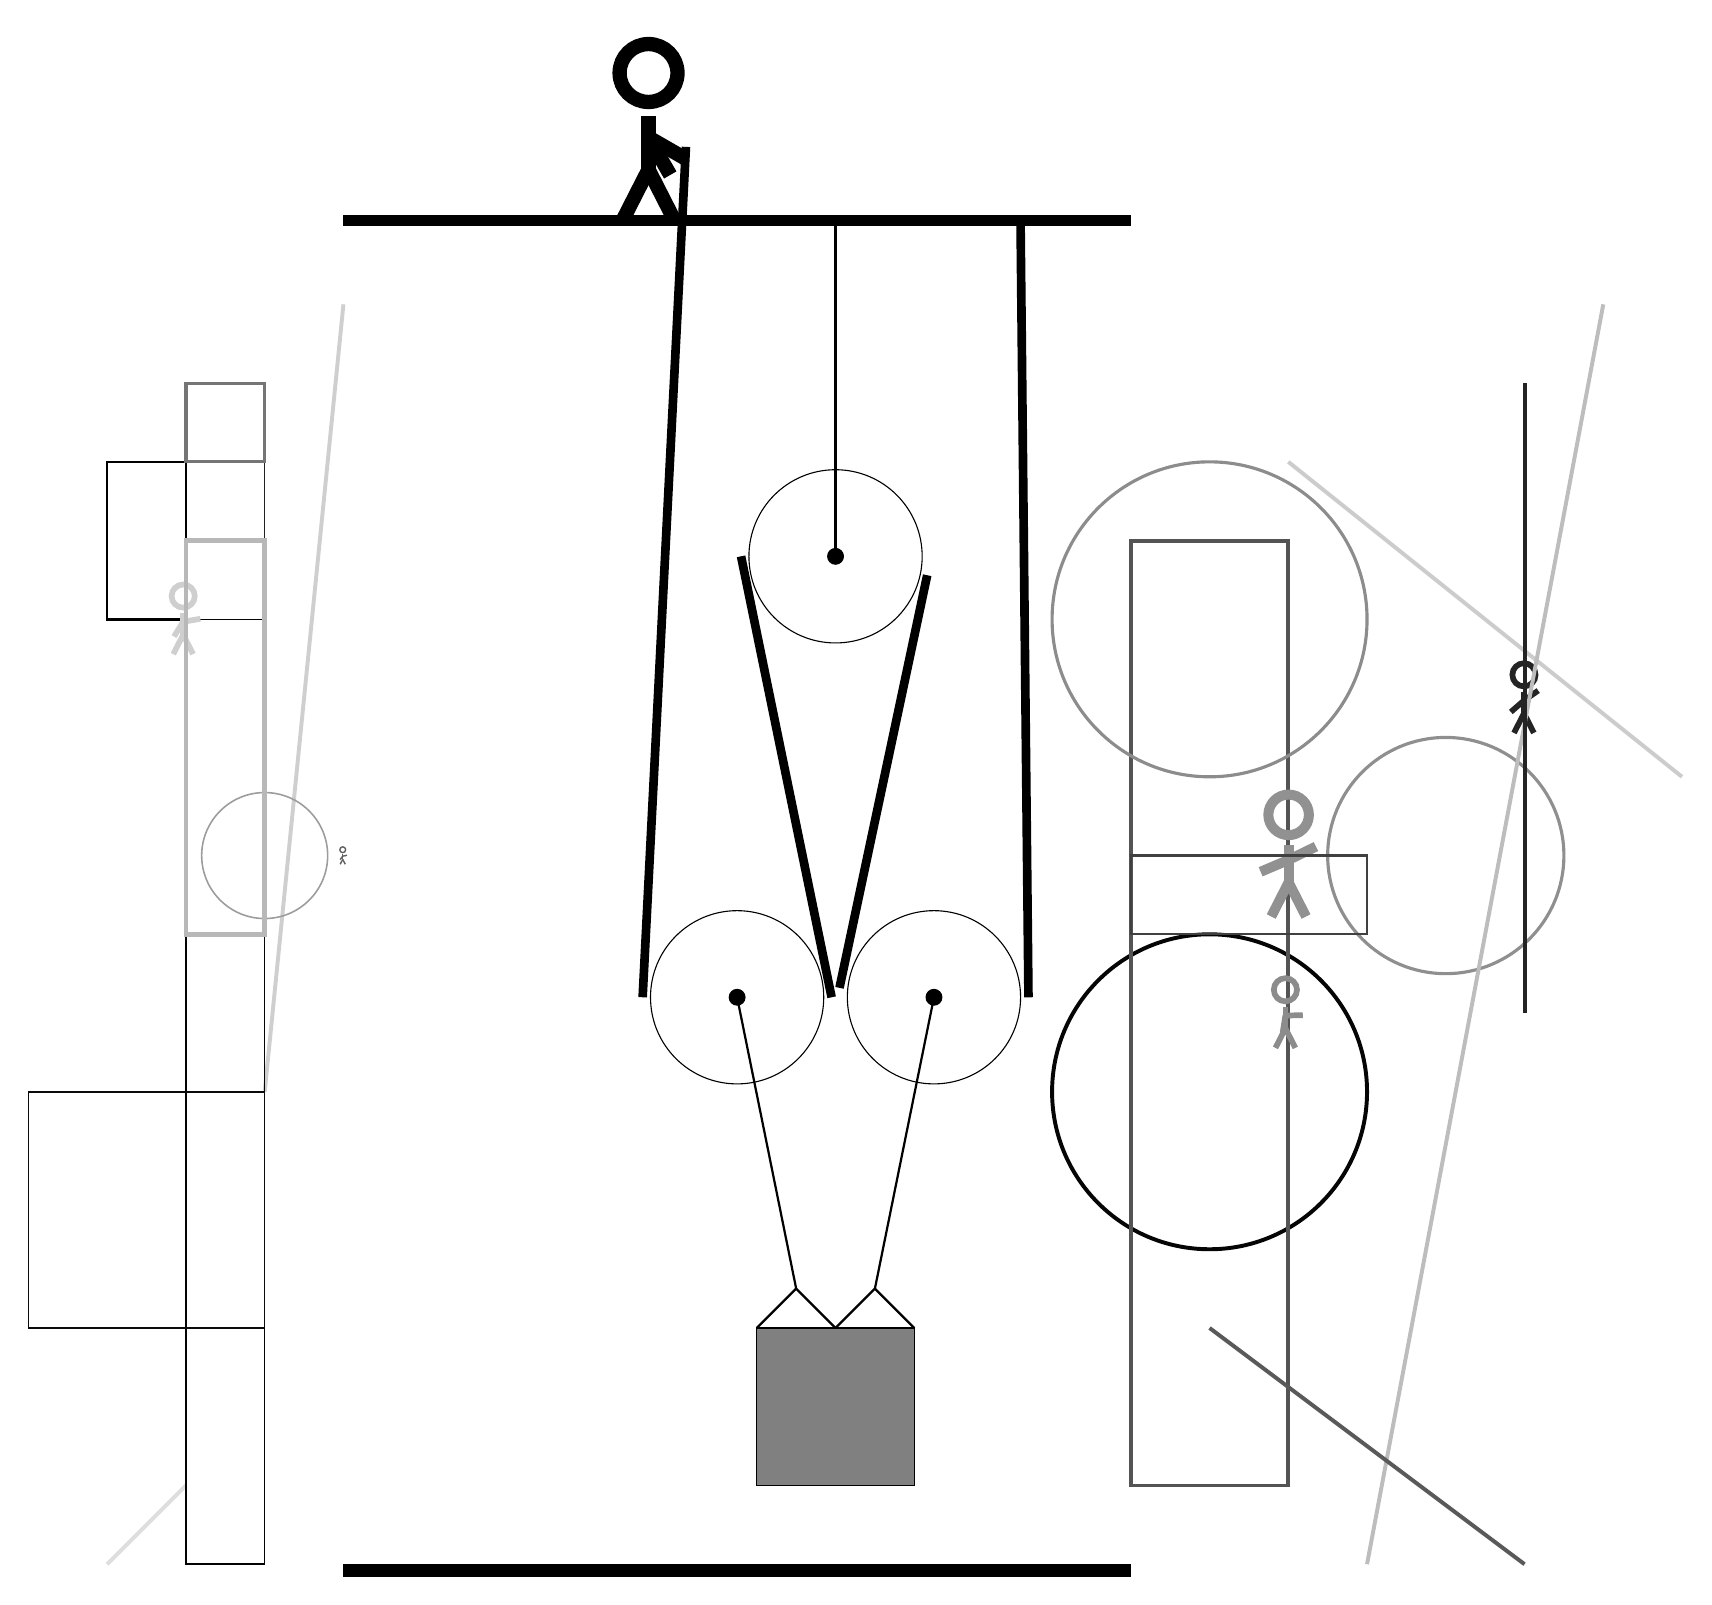
\begin{tikzpicture}
			%%%%% START %%%%%
			
			\draw[fill=black] (-4, 14) rectangle (6, 14.125);
			
			\draw (1, 4.2) circle (1.1);
			\draw[fill=black] (1, 4.2) circle (0.1);
			
			\draw (2.25, 9.8) circle (1.1);
			\draw[fill=black] (2.25, 9.8) circle (0.1);
			\draw[thick] (2.25, 9.8) -- (2.25, 14);
			
			\draw (3.5, 4.2) circle (1.1);
			\draw[fill=black] (3.5, 4.2) circle (0.1);
			
			\draw[thick] (3.5, 4.2) -- (2.75, 0.5);
			\draw[thick] (1, 4.2) -- (1.75, 0.5);
			\draw[thick]  (1.25, 0) -- (1.75, 0.5) -- (2.25, 0);
			\draw[thick]  (2.25, 0) -- (2.75, 0.5) -- (3.25, 0);
			\draw[fill=black!50] (1.25, 0) rectangle (3.25, -2);
			
			\draw[line width=1.1mm] (0.35, 15) --  (-0.2, 4.2);
			\centerarc[line width=1.1mm](1, 4.2)(180:360:1.2000000000000002);
			\draw[line width=1.1mm] (2.2, 4.2) -- (1.05, 9.8);
			\centerarc[line width=1.1mm](2.25, 9.8)(-20:180:1.2000000000000002);
			\draw[line width=1.1mm](3.414, 9.56) -- (2.3, 4.32);
			\centerarc[line width=1.1mm](3.5, 4.2)(160:360:1.2000000000000002);
			\draw[line width=1.1mm](4.7, 4.2) -- (4.6, 14);
			
			\node at (-0.07, 15.2) {\Strichmaxerl[10][120][-30]};
			
			\draw[line width=0.3mm, color=black!100] (-6, 11) rectangle (-7, 9);
			
			\draw[line width=0.5mm, color=black!13](-7, -3) -- (-6, -2);
			\draw [line width=0.5mm, color=black!98](7, 3) circle (2.0);
			\draw[line width=0.5mm, color=black!19](-4, 13) -- (-5, 3);
			\draw[line width=0.2mm, color=black!99] (-5, -3) rectangle (-6, 9);
			\draw[line width=0.2mm, color=black!87] (-5, 8) rectangle (-5, 11);
			\draw[line width=0.5mm, color=black!67] (6, 10) rectangle (8, -2);
			
			\node[line width=0.5mm, color=black!62] at (-4, 6) {\Strichmaxerl[1][53][12]};
			\node[line width=0.6mm, color=black!86] at (11, 8) {\Strichmaxerl[4][41][35]};
			\node[line width=0.7mm, color=black!19] at (-6, 9) {\Strichmaxerl[4][58][10]};
			
			\draw[line width=0.2mm, color=black!96] (-5, 3) rectangle (-8, 0);
			
			\draw [line width=0.2mm, color=black!39](-5, 6) circle (0.8);
			\draw [line width=0.4mm, color=black!45](7, 9) circle (2.0);
			
			\draw[line width=0.5mm, color=black!20](8, 11) -- (13, 7);
			\node[line width=0.2mm, color=black!45] at (8, 4) {\Strichmaxerl[4][81][1]};
			\node[line width=0.3mm, color=black!43] at (8, 6) {\Strichmaxerl[7][23][26]};
			
			\draw[line width=0.4mm, color=black!54] (-6, 11) rectangle (-5, 12);
			\draw [line width=0.4mm, color=black!44](10, 6) circle (1.5);
			\draw[line width=0.3mm, color=black!75] (6, 5) rectangle (9, 6);
			\draw[line width=0.6mm, color=black!28] (-5, 5) rectangle (-6, 10);
			\draw[line width=0.5mm, color=black!26](9, -3) -- (12, 13);
			
			\draw[line width=0.5mm, color=black!65](7, 0) -- (11, -3);
			\draw[line width=0.5mm, color=black!86](11, 12) -- (11, 4);
			
			\draw[fill=black] (-4, -3) rectangle (6, -3.15);
			
			%%%%% END %%%%%
		\end{tikzpicture}
	\end{figure}	
\end{document}